\documentclass{tufte-handout}
\usepackage{graphicx}
\graphicspath{ {./images/} }

%% use \begin{marginfigure} for figures on the side. \begin{figures} otherwise
\title{Notes on Pattern Recognition}
\author{Andres Ponce}

\begin{document}
\maketitle
\begin{abstract}
		Pattern Recognition is a subset of Machine Learning and Aritficial 
		Intelligence in general. It's concerned with analyzing data, extracting
		particular features or patterns from that data. We will discuss severl 
		methods for feature extraction, all the way to neural networks and 
		just touch on deep learning!
\end{abstract}

\section{Introduction}
Here, I am using the \texttt{tufte-latex} package for \LaTeX. I thought
the design looked quite nice and wanted to give it a shot! 

\section{Curve Fitting}
	\newthought{There exist} two main types of problems in the field of pattern 
	recognition. First, there is \textit{\textbf{regression}}, and
	there is \textit{\textbf{categorization}}. \footnote{\textbf{regression}
	problems deal with the mapping of an input vector to a continuous space,
	whereas \textbf{categorization} takes an input and places it in a finite 
	and discrete set of different categories.}

	The terms \textit{Artificial Intelligence, Machine Learning,} and 
	\textit{Pattern Recognition} all share common properties. PR $\land$ ML
	$\subset$ AI. ML atempts to make computers take in empirical data and 
	make decisions. AI, more broadly, tries to make computers perform actions
	that were usually thought to be exclusive to humans. 
	
	Some different types of PR problems involve \textbf{supervised} and
	\textbf{unsupervised} learning. \footnote{Their difference is whether their 
	target data is available when the problem begins, i.e. whether we know
	the correct answer.} There might be a couple of problems that better suit 
	un-supervised learning, such as:
	\begin{itemize}
		\item{\textbf{Clustering}}: Clustering involves finding patterns in the 
				data which more often resemble themselves rather than other data,
				i.e. finding similar patterns within the data. 
		\item{\textbf{Density Estimation}}: Here, we try and find the probability 
				density function given a set of points.\footnote{Remember the PDF
				only represents a probability density over a continuous interval.}
		\item{\textbf{Dimensionality Reduction}}: When multiple variables are involved
				in a problem, the space in which their solution exists rises exponentially
				for each new variable.\footnote{i.e. solving for three variables is exp. 
				harder than solving for two.} 
	\end{itemize}
	Although we can imagine supervised scenarios, IRL our model would probably have to find
	the solutions on its own. 

	We can imagine having a network actually \textit{generate} new data based on the patterns
	its seen before. For example, given many human faces, we could create a model that generates
	human faces which do not exist in reality. This would be the idea of a \textbf{Generative
	Adversarial Network}(GAN)\footnote{A GAN could have \textit{two} networks, one that generates
	the data and the other one that checks its validity.}

	Finallly, curve fitting! So, we have a polynomial function, whose generic form is
		\[ y(x,w)= w_{0}+w_{1}x+w_{2}x^{2}+...+ w_{M}x^{M} = \sum_{j=0}^{M}w_{j}x^{j}\]
	$M$ gives us the  order of the polynomial, and if I remember my algebra correctly, it 
	should have $M-1$ curves.  If M is too large, we \textit{overfit} and our function
	will have too many curves and not match the actual function all that well.

	$w$ gives us the value of the constant mulitplier, which can be found by minimizing the 
	\textbf{expectation} $E(w)$.\footnote{The expectation is like the average, the value 
	we should expect to see from a random variable.} This expectation is fiven by 
	\[E(w)=\frac{1}{2}\sum_{n=1}^{N} \{y(x_{n},w)-t_{n}\}^{2} \]
	Basically we want the difference between the value that our function gave us and the 
	acutal value of the function.

		\begin{marginfigure}
			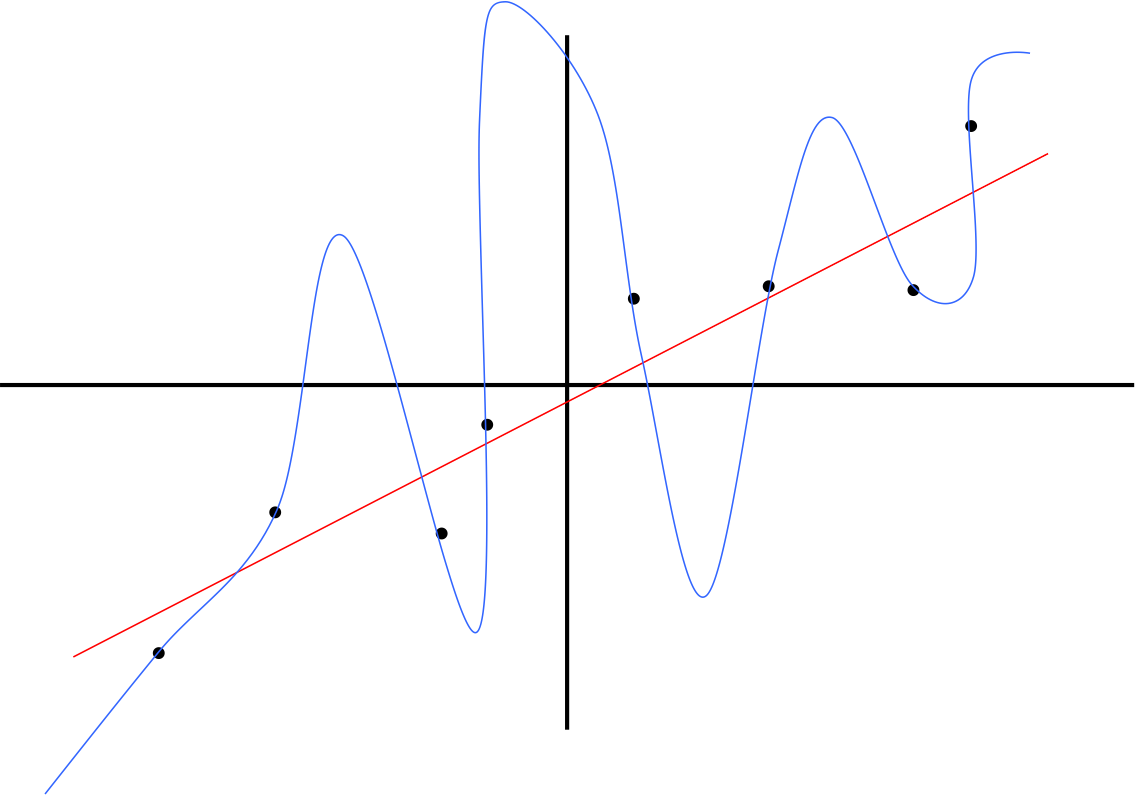
\includegraphics[width=\linewidth]{overfitting}	
			\caption{Overfitting leads to overly complex models. The blue line
				is our model.}
			\label{fig:overfitting}
		\end{marginfigure}
	Because we want to avoid overfitting, we introduce a weight term to our cost 
	function. In Figure \ref{fig:overfitting}, our model tries to overcompensate 
	because it tries to fit to every single data point, with all its discrepancies included. 
	Therefore, if we add a specific value to our cost function, it would encourage the model
	to choose a curve that works within the defined parameters and is not too complex. Our 
	new curve might be something like:
	\[ \tilde{E}(w)= \frac{1}{2} \sum_{n=1}^{N}\{y(x_{n},w)-t_{n}\}^{2}+\frac{\lambda}{2}\|w\|^{2}\]
	where $\|w\|^{2}=w^{T}w = \sum_{n=0}^{M}\omega_{n}^{2}$. We could also include a linear term
	for $w$, but with its quadratic version it would be a \textbf{ridge regression}. We will have 
	to choose our $w$ such that $\tilde{E}(w)$ is minimized, thus if we add a bigger term at the 
	end(quadratic), the value rises quicker and we'll choose a smaller $w$.

	\subsection{Probability}
		We need to review the fundamentals of probability before moving. 


		The \textbf{expectation} of a probability can be thought of as the average value of a 
		probability distribution, or the value that we should expect should we pick a random 
		value from the distribution; the value that the distribution revolves around. The main 
		idea is that we multiply all the possible values of $f(x)$ by the probability that 
		it is such a way. Thus, for a discrete distribution, the expectation is 
		\[ \mathbb{E}[f]= \sum_{x}^{}p(x)f(x)\]We replace the sum with an integral 
		for a continuous distribution.	


		The \textbf{variance} is the expected value that a random variable deviates from the 
		expected value. \footnote{\textbf{Variance} is the expected amount that the 
		expected amount differs from $f(x)$. 
		The value is squared so the expectation removes positive.}
		\[ var[f] = \mathbb{E}[(f(x) - \mathbb{E}[f(x)])^{2}]\]

		\textbf{Covariance} refers to the amount that two random variables vary together. The 
		\textbf{Gaussian Distribution} refers to a very complicated formula that describes a
		probability distribution.  There can be multivariate distributions that utilize a 
		Gaussian distribution, which has a \textbf{covariance matrix} for all the variables and
		how they relate to each other. 

	\subsection{Bayes's Theorem}
		This theorem relates the inverse conditional probability $p(w|D)$ with $p(D|w)$. 
		\[ p(w|D) = \frac{p(D|w)p(w)}{p(D)}\]
		Given the set of observations $D$, we can formulate how likely it was for a certain 
		coefficient $w$ to arise both before observing the data and after. \footnote{The 
		\textbf{prior probability} $p(w)$ of the parameter $w$ is its likelihood 
		before observing D. $p(D|w)$, the \textbf{likelihood function}, relates how likely
		the observations are given the parameter. It's gotten after observing $D$.} 
\section{Probability Distributions}
	\newthought{Suppose we have} an unfair coin that we are throwing in the air $n$ times. We would like
	to measure the probability of getting $x$ heads. The probability distribution would be:
	$p(x)=(p(x))^{x}(1-p(x))^{1-n}$. This is known as the \textbf{Bernoulli Distribution}

	Similar to the Bernoulli distribution, we might consider the \textbf{Binomial Distribution},
	where factor in the \textit{different} possible ways to draw M heads. The formula then becomes:
	\[ \textrm{Bin}(m|N,\mu) = {N\choose M}\mu^{m}(1-\mu)^{N-m}\]\footnote{This formula relates the 
	probability fo the \textit{combinations}, or possible orderings, in which $M$ events happen.}

	\subsection{The Beta Distribution}
	First, we have to talk about \textbf{prior distributions} and \textbf{posterior distributions}.
	These are $p(\theta)$ and $p(\theta|x)$, respectively.\footnote{The difference between the two is
	knowing the result of some variable $x$ which can influence the result. Together they are known as
	\textbf{conjugate distribution}.} 

	Together, these inform us as to how the probabilities for a random event and its complement 
	depend mutually on each other. The hyperparameters $a$ and $b$ can be considtered the amount
	of times that the observations for $x=1$ and $x=0$ have been observed.

	\newthought{This was in the textbook, not in the presentation}
\section{Regression}
	\newthought{If we remember}, when doing regression, we have a \textbf{basis function}.\footnote{
	A \textbf{basis function} is a function that allows us to reach any point within a given space.
	I think it might be similar to how you can reach any point in 3D with three orthogonal vectors?}
	Whatever approximation we wish to do would then probably be some sort of linear combination of the 
	original basis function.
	
	The basis function is of the form(we will describe the forms of $\phi$ below):
	\[ y=w_{0}+w_{1}\phi_{1}(x)+...+w_{M-1}\phi_{M-1}(x)\]
	However, as with overfitting, the basis function will not necessarily allow you to automatically 
	reach all the space at first. However, since linear functions will just allow a straight line, then 
	we cannot use it always. Some examples of basis functions include:

	The key to understand is the basis function $\phi$. Because we have an input vector $\{X\}$ with n
	elements, each of the  $x_{n}$ will have to be passed through $\phi$.
	\begin{itemize}
			\item \textbf{Polynomial}: These functions are of the form:
					\[ \phi_{j}(x)=x^{j}\]
			\item \textbf{Gaussian}: governed by $\mu_{j}$ and $s$.\footnote{Notice how $\mu_{j}$
					will determine how big our numerator and denominator are, i.e. the expected value
					tells us more than anything what to expect.}	
					\[ \phi_{j}(x) = \textrm{exp}\{ -\frac{(x-\mu_{j})^{2}}{2s^{2}} \}\]
			\item \textbf{Sigmoidal}:
			\[ \phi_{j}(x) = \phi(\frac{x-\mu_{j}}{s}) \textrm{ where } \phi(a) = \frac{1}{1+\textrm{exp}(-a)}\]
	\end{itemize}

	In the figure below, $t$ refers to the \textbf{target vector}, which is the result of the actual
	function $y(x,w)$ and a random gaussian nose $\epsilon$
	\footnote{Essentially, this formula says that the 
	likelihood of a given target vector $t$
	given a certain input vector $x$, parameter $w$, and precision $\beta$ is the product 
	of the normal distribution of each member in $t$. This makes sense since the probability 
	that our target vector is a certain way would depend on the normal distribution. And since 
	every $x$ is independently and identically distributed, having the product of all of them
	should give the correct overall likelihood. Right? :) }
	\[ p(t|x,w,\beta ) = \prod_{n=1}^{N}\aleph(t_{n}|w^{T}\phi(x_{n}),\beta^{-1}) \]

	Often times, to find the maximum of the likelihood function, we instead take its natural
	logarithm. We do this because the function itself is \textbf{monotonically increasing},
	meaning that maximizing the likelihood function is equivalent to maximizing the 
	\textbf{log likelihood function}.
	\subsection{Least Squares}
	The idea behind a \textbf{Least Squares Approximation} is to take the difference between the 
	function value and the one our model gives us. We take this difference (squared to maintain a
	positive number) and try to minimize over the whole sum of errors. Then, optimality would involve
	minimizing the log likelihood function.

	However, least squares solutions can also suffer from \textbf{overfitting}, so we can add
	a \textbf{regulartization}. This term ensures that our approach does not overfit the actual
	answer again. As metnitoned, we can add a linear term or a quadratic term. The general form 
	for a good equalizer might be:\footnote{where $t$ is target vector,$w$ would be the 
	parameter matrix? $\phi$ is the basis function}
	\[ \frac{1}{2}\sum_{n=1}^{N}\{t_{n}-w^{T}\phi(x_{n})\}^{2}+ \frac{\lambda}{2}\sum_{j=1}{M}|w_{j}|^{q} \]

	\subsection{Multiple Outputs}
	Suppose we have target vector with multiple components. The way to find the best coefficients would
	be to have either multiple basis functions or to estimate the components of $\textbf{t}$. This would
	be equivalent to $K$ indpendent regresion problems for $K$ dimensions.
	\subsection{Maximum a posterior}
	In regression problems, both the prior and posterior probabilities are Gaussian.
	Thus\footnote{$m_{0}$ and $S_{0}$ are the mean and covariance matrix respectively.} 
	\[ p(w) = \aleph(w,m_{0},S_{0})\]
	and 
	\[ p(w|\textbf{t}) = \aleph(w|m_{N},S_{N})\]
	are both Gaussian in nature.
	
	After that, we finally start using the predictive function $y(x,w)$ to guess the points.\footnote{Remember
	this function takes the parameters and multiplies them by the basis function, and adds some Gaussian
	noise just cuz.}
	\begin{figure}[t]		
			\centering
			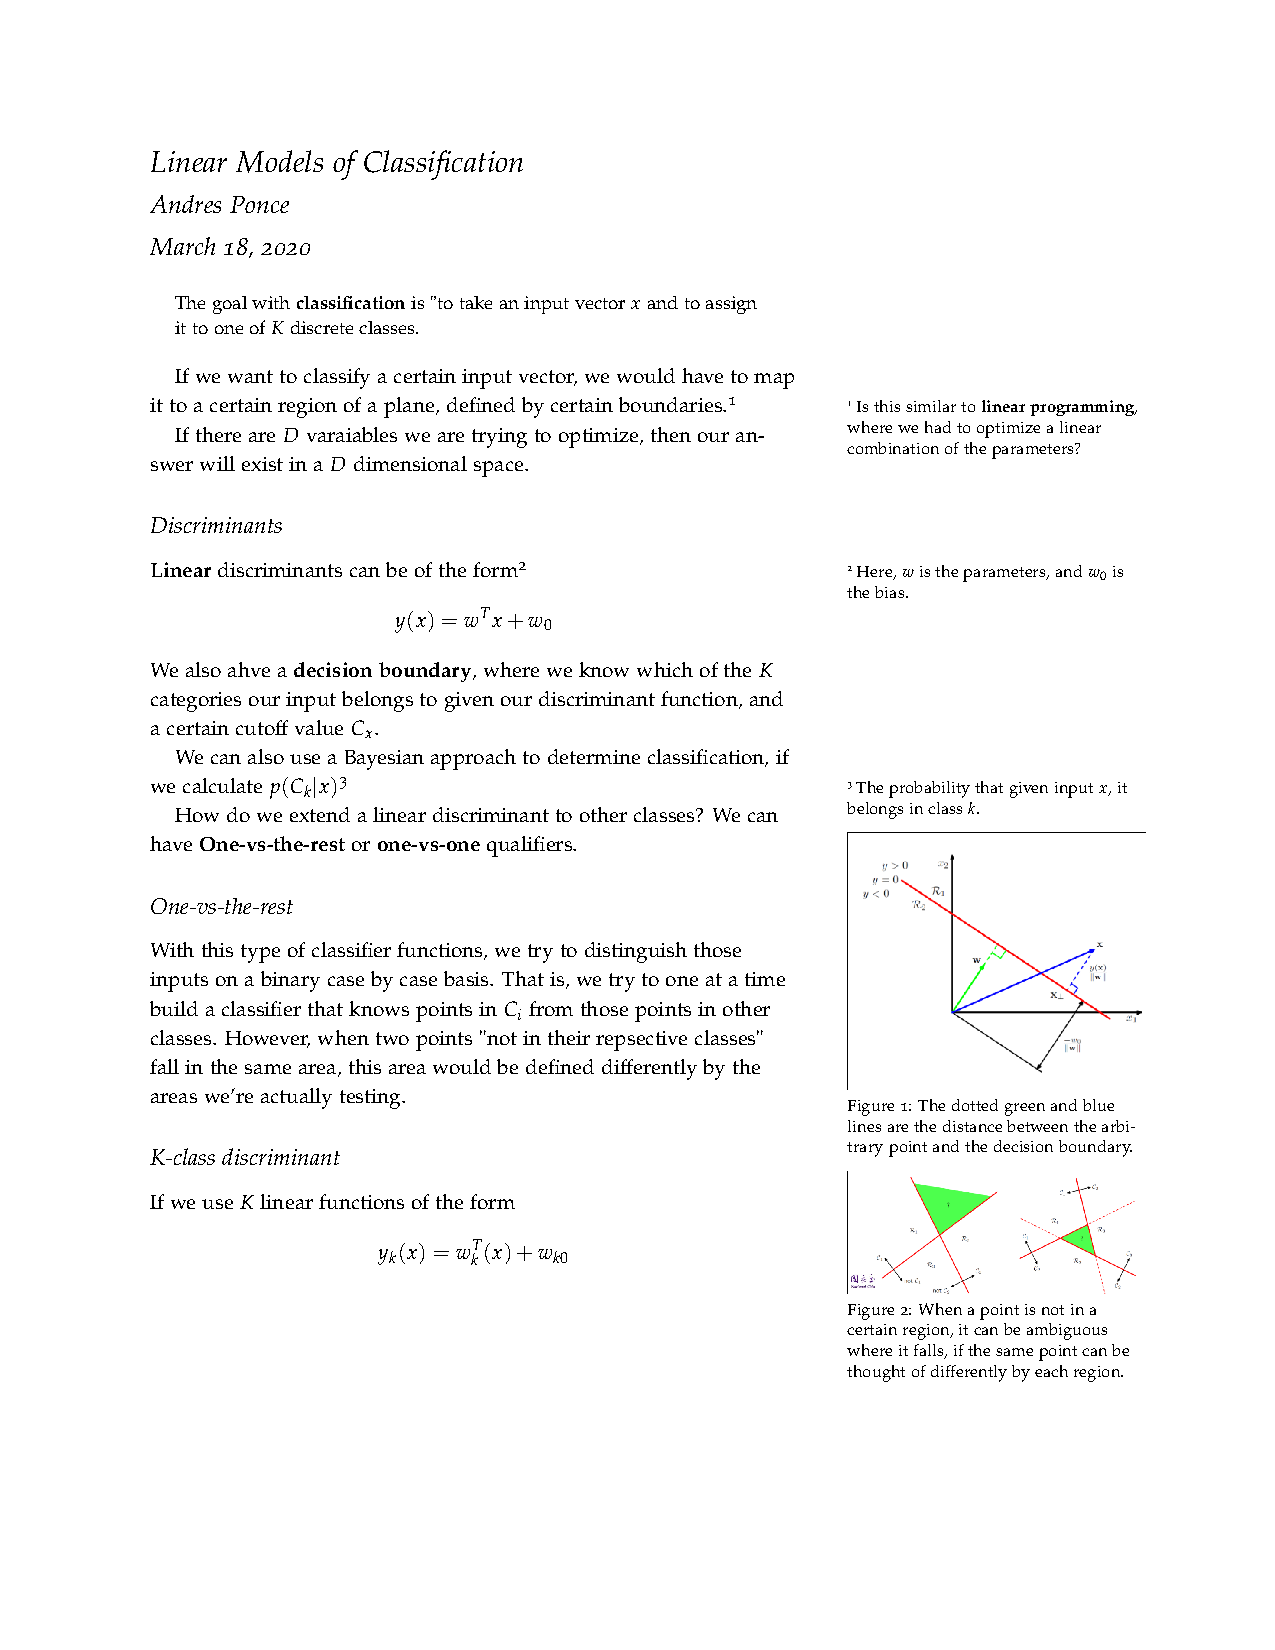
\includegraphics[width=\textwidth]{regression}\\
			\caption{The red line is our predictive function; the green is our actual function
				which we don't know, and the red area reps. 1 standard deviation from the function
				value at each point.}
	\end{figure}
\end{document}
